\chapter{Image recognition for IBD reconstruction with the SPMT system}
\label{sec:jcnn}

\epigraph{\textit{Dave} - Give me the position and momentum, HAL. \\
\textit{HAL} - I'm afraid I can't do that Dave. \\
\textit{Dave} - What's the problem ? \\
\textit{HAL} - I think you know what the problem is just as well as I do. \\
\textit{Dave} - What are you talking about, HAL? \\
\textit{HAL} - $\sigma_x \sigma_p \geq \frac{\hbar}{2}$}

As explained in chapter \ref{sec:juno}, JUNO is an experiment composed of two systems, the Large Photomultiplier (LPMT) and the Small Photomultiplier (SPMT). Both of the system observe the same physics event inside of the same medium but they differ in their photo-coverage, respectively 75.2\% and 2.7\%, their dynamic range (see section \ref{sec:juno:LPMT}), a thousands versus a few dozen, and their front-end electronics (see section \ref{sec:juno:LPMT}).

They are complementary in their strengths and weaknesses and support each other. One important point is their differences in expected resolution, the LPMT system outperform largely the SPMT system but is subject to effects such as charge  non linearity \cite{juno_collaboration_calibration_2021} that could bias the reconstruction, effect that the SPMT system is impervious to. This topic will be studied in more detail in chapter \ref{sec:joint_fit}. Also, due to the dynamic range of the LPMT, in case of high energy and high density event such as core-collapse supernova, the LPMT system could saturate and the lower photo-coverage become a benefit.

Thus, although event reconstruction algorithm and physics analysis combines both LPMT and SPMT systems, individual approach are key studies to understand the detector and ensure their reliability. This topic will also be studied in more details in chapter \ref{sec:joint_fit}. The subject of this chapter is to propose a machine learning algorithm for the SPMT reconstruction based on Convolutional Neural Network (CNN).

\section{Motivations}

% -------------- Plan for motivation section ----------------
%\begin{itemize}
%  \item Promise of machine learning -> Exploit raw data
%  \item Victor already done reco for SPMT
%  \item Can CNN give similar results ? Better results ?
%  \item Multiple reco methods good for reconstruction
%  \item Comparison, difference in behavior
%\end{itemize}

As explained in chapter \ref{sec:ml}, Machine Learning (ML) algorithms shine when modeling highly dimensional data from a given dataset. In our case, we have access to complete monte-carlo simulation of our detector to produce arbitrary large datasets that could represent multiple years of data taking.
Ideally ML algorithms would be able to consider the entirety of the information in the detector and converge on the best parameters to yield optimal results, while classical methods where the algorithms could be biased by the prior knowledge of the detector and physics processes. To study this potential phenomena, we will compare our machine algorithm to a classical reconstruction method developed for energy and vertex reconstruction \cite{lebrin_towards_2022}.

We have access to a very detailed simulation of the detector (section \ref{sec:juno:software}) that will allow us to simulate arbitrary large dataset of data while giving access to the all the physics parameters of the event. Those parameters include the target of our reconstruction algorithms: the vertex and position at with the event happened. As introduced above, we hope that the ML algorithm will be able to used all the informations in the event, meaning that potential mismodelings in our simulation could be exploited by the algorithm. This specific subject will be studied in chapter \ref{sec:janne}.

\section{Method and model}
% --------------- Plan for method and model -----------------
%\begin{itemize}
%  \item JUNO is an array of sensor following a quasi uniform and istropic geometric repartition -> Basically pixels -> Image
%  \item CNN is gud for image processing (cite a lot of things)
%  \item Details the architecture (Inspired from VGG 16)
%    \begin{itemize}
%      \item Convolutional layers
%      \item Pooling layers -> Twice the channels when pooling by 2 -> Keep the same "amount" of information
%      \item Dropout (introduce overtraining, maybe introduce overfitting in ML chapter ?)
%      \item Vectorization fed to FCDNN
%    \end{itemize}
%\end{itemize}

One of simplest way to look at JUNO data is to consider the detector as an array of geometrically distributed sensors on a sphere. Their repartition is almost homogeneous, on this sphere surface providing an almost equal amount of information per unit surface on this sphere. It is then tempting to represent the detector as a spherical image with the PMT in place of pixel. Two events with two different energy or position would produce two different images.

The most common approach in machine learning for image processing and image recognition is the Convolutional Neural Network (CNN). It is widely used in research and industry \cite{simonyan_very_2015, ciresan_multi-column_2012, abbasi_convolutional_2021, maksimovic_cnns_2021} due to its strengths (see section \ref{sec:ml:cnn}) and has proven its relevance in image processing.

Some CNN are developed to process spherical images \cite{cohen_spherical_2018} but for the sake of simplicity and as a first approach we decided to go with a planar projection of the detector, approach that has proven its efficiency using the LPMT system (see section \ref{sec:juno:ml}). The details about this planar projection will be discussed in section \ref{sec:jcnn:data}.

\begin{figure}[ht]
  \centering
  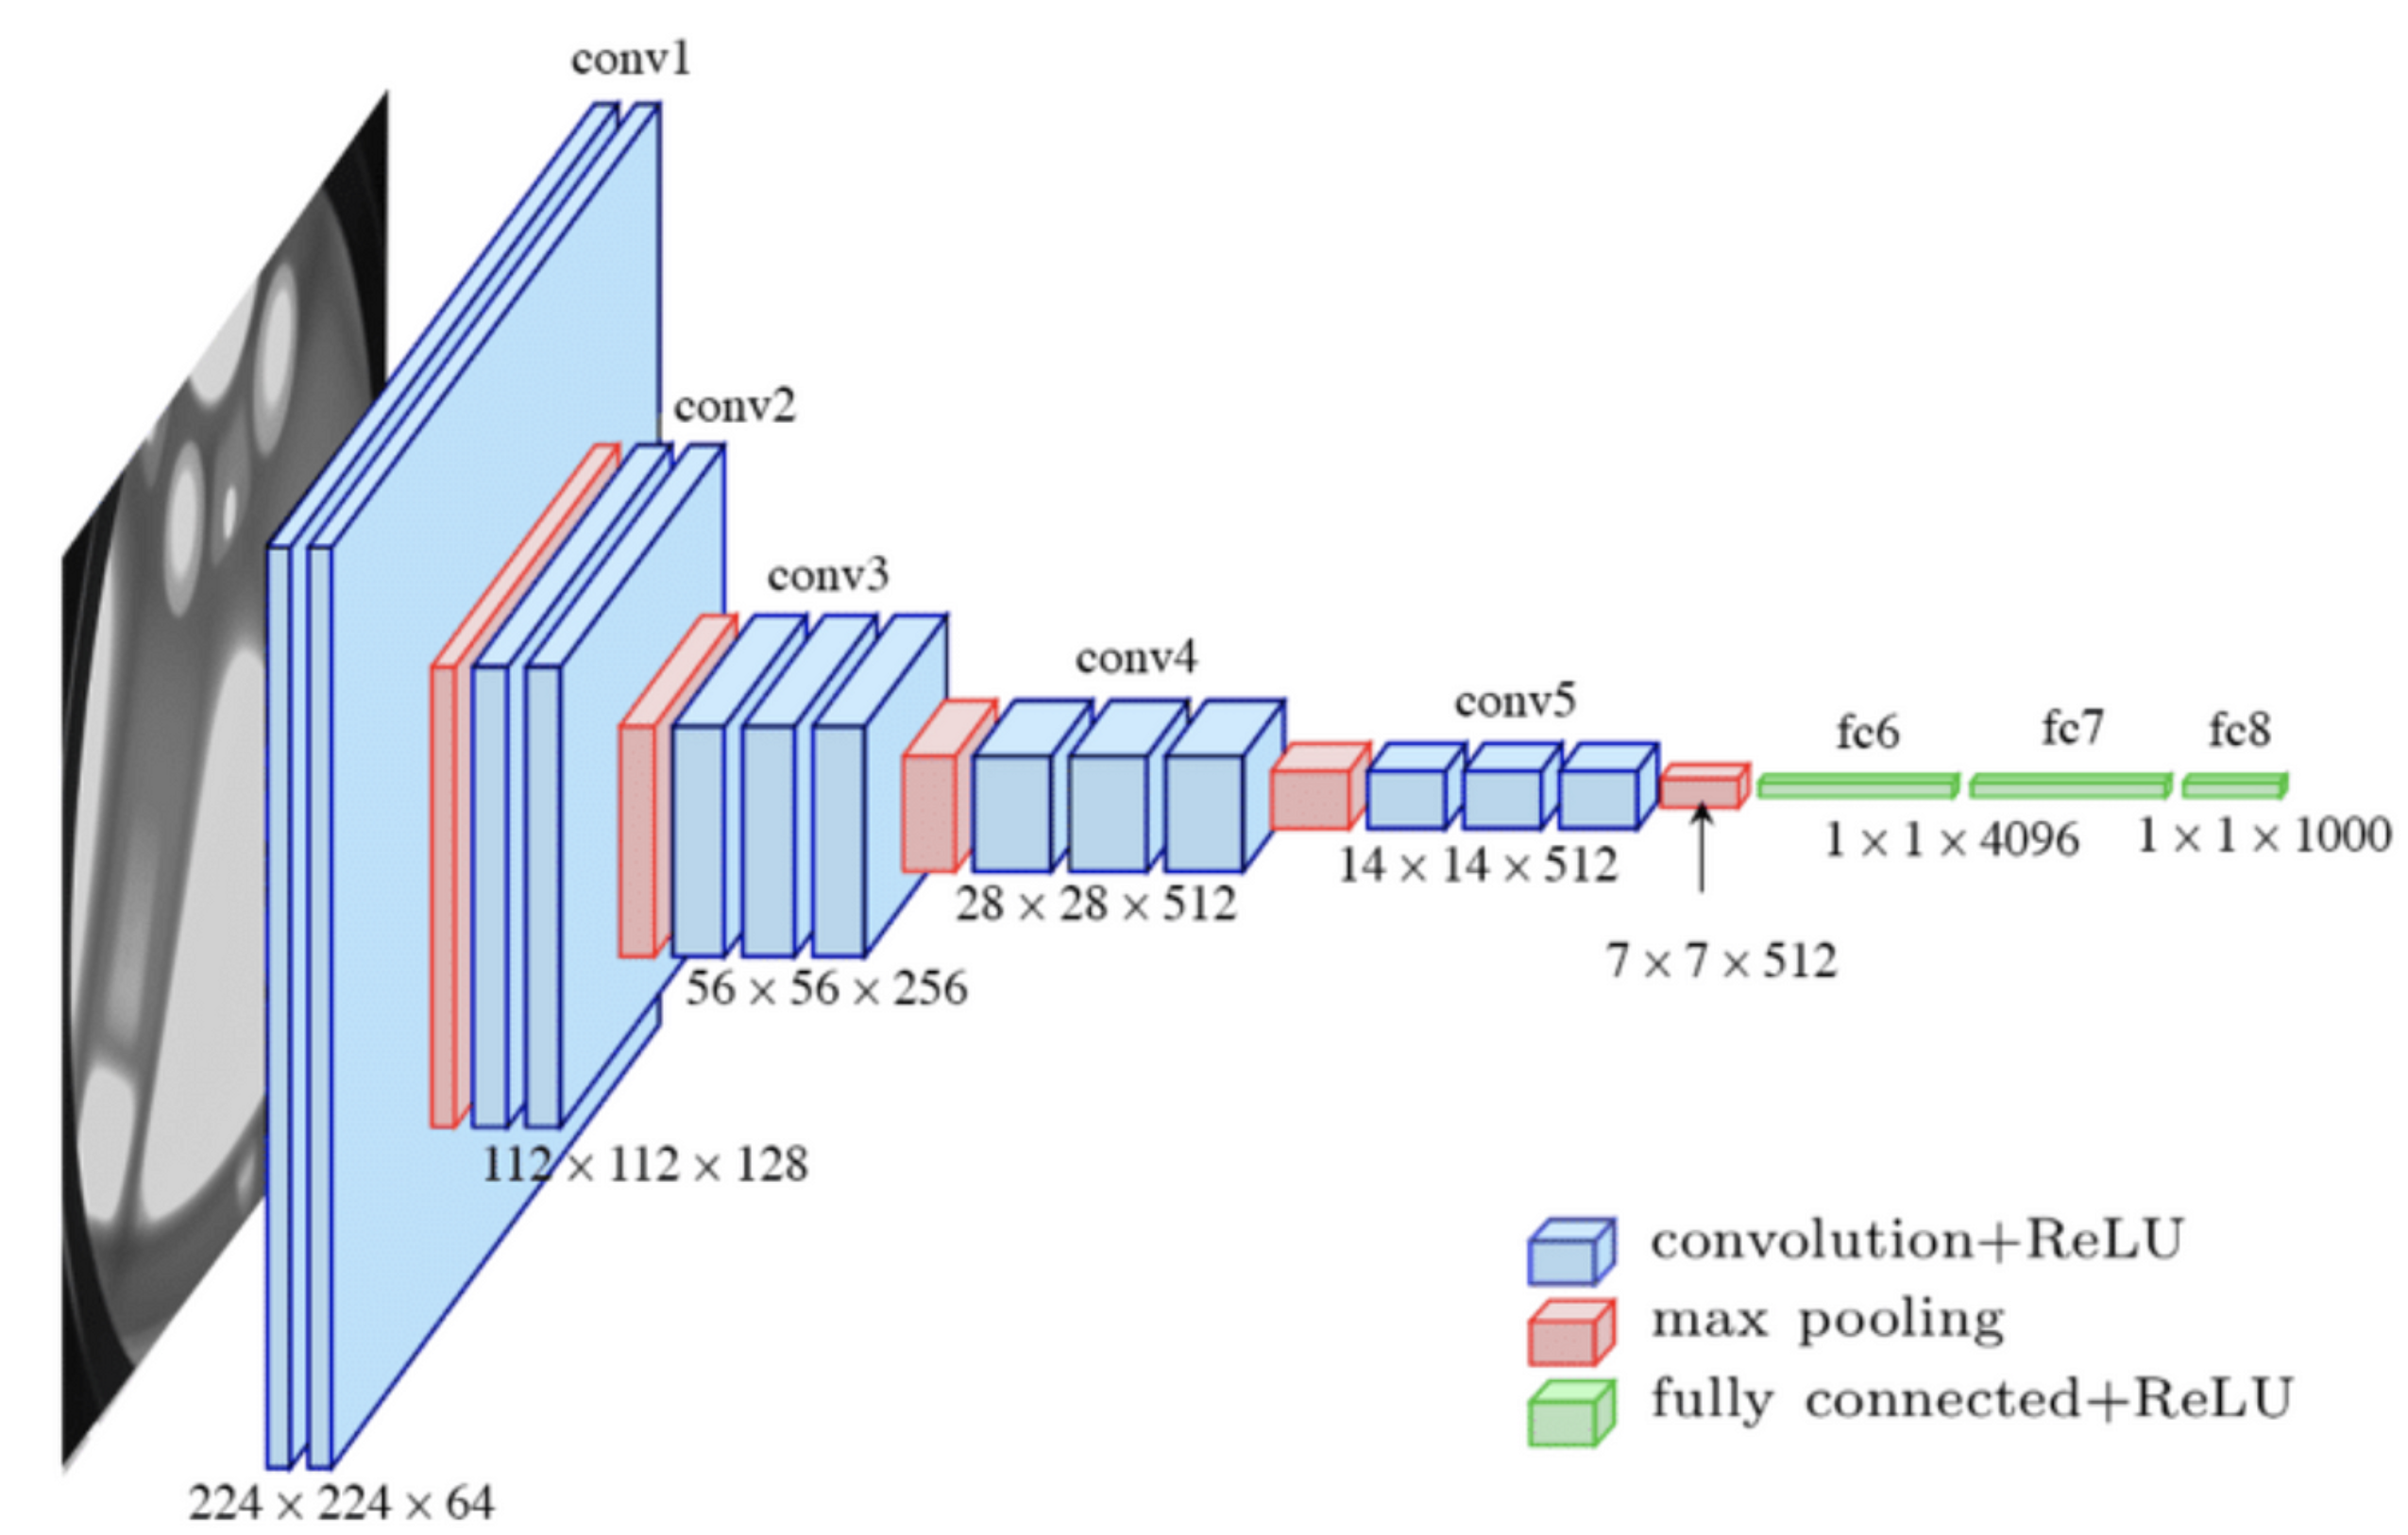
\includegraphics[height=6cm]{images/jcnn/vgg16.png}
  \caption{Graphic representation of the VGG-16 architecture, presenting the different kind of layer composing the architecture.}
  \label{fig:jcnn:vgg16}
\end{figure}

\subsection{Model}
\label{sec:jcnn:model}

The architecture we use is derived from the VGG-16 architecture \cite{simonyan_very_2015} illustrated in figure \ref{fig:jcnn:vgg16}. We define a set of hyperparameters that will define the size, complexity and computational power of the NN. The chose hyperparameters are detailed below and their values are presented in table \ref{tab:jcnn:hyper}.
\begin{itemize}
  \item $\mathbf{N_{blocks}}$: the number of convolution blocks, a block being composed of two convolutional layers with $3\times3$ filters using ReLU activation function, a $3\times3$ max-pooling layer (except for the last block) and a dropout layer.
  \item $\mathbf{N_{channels}}$: The number of channels in the first block. The number of channels in the subsequent blocks are calculated using $N^i_{channels} = 2^{i} * N_{channels}, i \in [1..N_{blocks}]$.
  \item \textbf{FCDNN configuration}: The result of the last convolution layer is flattened then fed to a FCDNN. Its configuration is expressed as a sequence of fully connected linear layer using the PReLU activation function. For example $2 * 1024 + 2 * 512$ is the sequence of 2 layers with a width of 1024 followed by 2 other layers with a width of 512. Finally the last layer is a 4 neurons wide linear layers without activation function. Each neurons of the last layer represent a component of the interaction vertex: Energy, X, Y, Z.
  \item \textbf{Loss}: The loss function. In this work we study two different loss function $(E+V)$ and $(E_r + V_r)$ detailed below.
\end{itemize}

\begin{align}
  (E+V)(E, x, y, z) &= \bigg\langle (E - E_{true})^2 + 0.85 \sum_{\lambda \in [x, y, z]} (\lambda - \lambda_{true})^2 \bigg\rangle \\
  (E_r + V_r)(E, x, y, z) &=  \bigg\langle \frac{(E - E_{true}) ^ 2}{E_{true}} + \frac{10}{R} \sum_{\lambda \in [x, y, z]} (\lambda - \lambda_{true})^2 \bigg\rangle
\end{align}
where $R$ is the radius of the CD. With the energy in MeV and the distance in meters, we use the factor 0.85 and 10 to equilibrate the two term of the loss function so they have the same magnitude.
\begin{itemize}
  \item The loss function $(E+V)$ is close to a simple Mean Squared Error (MSE). MSE is one of the most basic loss function, the derivative is simple and continuous in every point. It is a strong starting point to explore the possibility of CNNs.
  \item $(E_r + V_r)$ can be see as a relative MSE.
\end{itemize}
The idea is that: due to the inherent statistic uncertainty over the number of collected Number of Photo Electrons (NPE), the absolute resolution $\sigma (E - E_{true})$ will be larger at higher energy than at low energy. But we expect the \textit{relative} energy resolution $\frac{\sigma(E - E_{true})}{E_true}$ to be smaller at high energy than lower energy as illustrated in figure \ref{fig:juno:rec:qtmle}. Because of this, by using simple MSE the most important part in the loss come from the high energy part of the dataset whereas with a relative MSE, the most important become the low energy events in the dataset. We hope that by using a relative MSE, the neural network will focus on low energy events where the reconstruction is considered the hardest part of the dataset.


On top those generated models, we define 4 hand tailored models:
\begin{itemize}
  \item ``gen\_0'': $N_{blocks} = 4$, $N_{channels} = 64$, FCDNN configuration: $1024 * 2 + 512 * 2$, Loss $\coloneq E+V$
  \item ``gen\_1'': $N_{blocks} = 4$, $N_{channels} = 64$, FCDNN configuration: $1024 * 2 + 512 * 2$, Loss $\coloneq E_r+V_r$
  \item ``gen\_2'': $N_{blocks} = 5$, $N_{channels} = 64$, FCDNN configuration: $4096 * 2 + 1024 * 2$, Loss $\coloneq E+V$
  \item ``gen\_3'': $N_{blocks} = 5$, $N_{channels} = 64$, FCDNN configuration: $4096 * 2 + 1024 * 2$, Loss $\coloneq E_r+V_r$
\end{itemize}

\begin{table}[ht]
  \centering
  \begin{tabular}{ | c | c | }
    \hline $N_{blocks}$ & \{2, 3, 4\} \\
    \hline $N_{channels}$ & \{32, 64, 128\} \\
    \hline
    \multirow{4}{*}{FCDNN configurations} & 2 * 1024 \\
                                        & 2 * 2048 + 2 * 1024 \\
                                        & 3 * 2048 + 3 * 512 \\
                                        & 2 * 4096 \\
    \hline
    Loss & \{$E+V$, $E_r + V_r$\} \\
    \hline
  \end{tabular}
  \caption{Sets of hyperparameters values considered in this study}
  \label{tab:jcnn:hyper}
\end{table}

Each combination of those hyperparameters (for example $(N_{blocks} = 2, N_{channels} = 32, \mathrm{FCDNN} = (2 * 1024), \mathrm{Loss} = (E+V))$), subsequently designated as configurations, is then tested and compared to each other over an analysis sample. We cannot use the mean loss because we consider multiple loss functions, there is no guarantee that comparison of their numerical value will be meaningful. We use multiple observables to rank the performances of each configuration:
\begin{itemize}
  \item The mean absolute energy error $\langle E \rangle = \langle | E - E_{true} | \rangle$. It is an indicator of the energy bias of our reconstruction.
  \item The standard deviation of the energy error $\sigma E = \sigma (E - E_{true})$. This the indicator on our precision in energy reconstruction.
  \item The mean distance between the reconstructed vertex and the true vertex $\langle V \rangle = \langle | \vec{V} - \vec{V}_{true} | \rangle$. This an indicator of the bias and precision of our vertex reconstruction.
  \item The standard deviation of the distance between the true and reconstructed vertex $\sigma V = \sigma |\vec{V} - \vec{V}_{true}|$. This is an indicator if the precision in our vertex reconstruction.
\end{itemize}

The models were developped in Python using the pytorch framework \cite{ansel_pytorch_2024} using  NVIDIA A100 \cite{noauthor_nvidia_nodate-1} and NVIDIA V100 \cite{noauthor_nvidia_nodate-2} gpus. The A100 was split in two so for those training the accessible gpu memory was 20 Gb making it impossible to train somes of the architecture due to memory consumption.

The training of one model takes between 4h and 15h depending of its size, overall training the full 72 model takes around 500 GPU hours. Even with parallel training, this random search hyper-optimisation was time consuming.


%Indeed, let's say we consider error on each of the component as random variable following a normal distribution. We allow ourself to use this representation as our signal possess a strong statistical uncertainty in NPE that follow a Poisson law, i.e. a Gaussian law $\mathcal{N}$ when NPE is high enough which is the case for our signal. So following:
%\begin{equation}
%  \Delta V = |\vec{V} - \vec{V}_{true}| = \sqrt{\Delta X^2 + \Delta Y^2 + \Delta Z^2}; ~ \Delta X, \Delta Y, \Delta Z \sim \mathcal{N}
%\end{equation}
%then
%\begin{equation}
%  \Delta V \sim \chi
%\end{equation}
%where $\chi$ is a Chi law which probability density function is different from 0 only in $\mathbb{R}^+$

\subsection{Data representation}
\label{sec:jcnn:data}
%\begin{itemize}
%  \item Data is 240x240 images
%    \begin{itemize}
%      \item Following $\theta$ and $\phi$ distribution, explain the coordinate system of JUNO
%      \item Optimized for $\approx$ 1 SPMT/pixel
%      \item 1 Charge channel
%      \item 1 Time channel
%    \end{itemize}
%  \item Discuss data format
%    \begin{itemize}
%      \item Empty pixel ? -> $Q = 0$, $T = 0$, what does it means/says ? 0 = no signal in a way
%      \item Image distortion
%        \begin{itemize}
%          \item \textbf{Maybe speak of this in the conclusion ?} Could be done in two step:
%          \item 1. Reconstruct $\theta$ and $\phi$
%          \item 2. "Rotate" the image so the event is at the center of the image -> Prevent distortion + reconstruction E and R become pseudo rotational invariant (as they should be)
%        \end{itemize}
%    \end{itemize}
%\end{itemize}

This data is represented as $240 \times 240$ images, equivalent to third order tensor, with a charge $Q$ channel and a time $t$ channel. The SPMTs are then projected on the plane as illustrated in figure \ref{fig:jcnn:pmt_rep}. The $x$ position is proportional to $\theta$ and the $y$ position is defined by $\phi \sin{\theta}$ in spherical coordinates. $\theta = 0$ is defined as being the top of the detector and $\phi = 0$ is defined as an arbitrary direction in the detector. In practice, this is the $\phi = 0$ given by the MC simulation.

\begin{align}
  x &= \bigg\lfloor \frac{\theta \cdot H}{\pi} \bigg\rfloor, ~ \theta \in [0, \pi] \\
  y &= \bigg\lfloor \frac{(\phi + \pi) \sin{\theta} \cdot W}{2\pi}\bigg\rfloor, ~ \phi \in [-\pi, \pi], ~ \theta \in [0, \pi]
\end{align}
where $H$ is the height of the image, $W$ the width of the image and $(0,0)$ the top left corner of the image.

When two SPMTs are in the same pixel, the charges are summed and the lowest of the hit-time is chosen. The SPMTs being located close to each other, we expect the time difference between two successive physics signals, two photons being collected, to be small. The first hit time is chosen because it can be considered as the relative propagation time of the photons that went the "straightest", i.e. that went under the less perturbation of the two. The only potential problem in using this first time come from the Dark Noise (DN). Its time distribution is uniform over the signal and could come before a signal hit on the other SPMT in the pixel. In that case, the time information in the pixel become irrelevant and we lose the timing information for this part of the detector.
As illustrated in figure \ref{fig:jcnn:pmt_rep} the dimension have been chosen optimized so that at most two SPMTs are in the same pixel while keeping the number of empty pixels relatively low to prevent this kind of issue.

While it could be possible to use larger images (more pixel) to prevent overlapping, keeping image small images gives multiple advantages:
\begin{itemize}
  \item As presented in section \ref{sec:jcnn:model}, the convolution filter we use are $3 \times 3$ convolution filter, meaning that if SPMTs would be separated by more that one pixel, the first filter would only see one SPMT per filter. This behavior would be kind of counterproductive as the first convolution block would basically be a transmission layer and would just induce noise in the data.
  \item It keep the network relatively small, while this do not impact the convolution layers, the flatten operation just before the FCDNN make the number parameters in the first layer of it dependent on the size of the image.
  \item It reduce the number of empty pixel in the image.
\end{itemize}
The question of empty pixel is an important question in this data representation. Their is two kind of empty pixel in the data.

The first kind is pixel that contain a SPMT but the SPMT did not get hit nor registered any dark noise during the event. In this case, the charge channel is zero, which have a physical meaning but then come the question of the time layer. One could argue that the correct time would be infinity (or the largest number our memory allows us) because the hit ``never'' happened, so extremely far from the time of the event. This cause numerical problem as large number, in the linear operation that are happening in the convolution layers, are more signifiant than smaller value. We could try to encode this feature in another way but no number have any significance due to our time being relative to the trigger of the experiment so $-1$ for example is out of question. Float and Double gives us access to special value such as NaN (Not a Number) \cite{noauthor_ieee_2019} but the behavior is to propagate the NaN which leaves us with NaN for energy and position. We choose to keep the value 0 because it's the absorbing element of multiplication, absorbing the ``information'' of the parameter it would be multiplied by. It also can be though as no activation in the ReLU activation function.

The second kind of pixel is pixel that do not represent parts of the detector such as the corners of the images. The question is basically the same, what to put in the charge and the time channel. The decision is to set the charge and time at 0 following the reasoning presented above. Its important to keep in mind that the fact that a part of the detector that has not been hit is also an information: There is no signal in this part of the detector. This problematic will be explored in more details in chapter \ref{sec:jgnn}.

Another problematic that happens with this representation, and this is not dependent of the chosen projection, is the deformation in the edges of the image and the loss of the neighbouring information in the for the SPMTs at the edge of the image $\phi \sim 180^\circ$. This deformation and neighbouring loss could be partially circumvented as explained in section \ref{sec:jcnn:prospect}

\subsection{Dataset}
% 1 Millions MC e+ events for training (900k for train, 50k for validation and 50k for test)
%   \begin{itemize}
%     \item MC for the moment, will need to retrain with mix of calibration data (Good question, is the CNN PID agnostic ?)
%     \item 47 IBD/day -> 1M event is 21k days of data (for reference, 6 years of data is 94k events)
%     \item Events are "optimistic"
%       \begin{itemize}
%         \item No pile-up
%         \item w/o neutrons
%         \item time window is decided by electronics
%       \end{itemize}
%   \end{itemize}


In this study we will discuss two datasets of one millions events:
\begin{itemize}
  \item \textbf{J21}: The first one comes from the JUNO official mc simulation J21v1r0-Pre2 (released the 18th August 2021). This historical version is the one on which the NN the classical algorithm presented in \cite{lebrin_towards_2022} was developped. This dataset is used as a reference for comparison to classical algorithm. The data in this dataset is \textit{detsim} level (see section \ref{sec:juno:software}), so where only the physic is simulated. The charge and time biases and uncertainties are added using toy MC adjusted using \cite{cao_mass_2021, abusleme_mass_2022}. The time window is not based on a selection algorithm but is defined as the first PMT hit for $t_0$ up to $t_0 + 1000$ ns.
  \item \textbf{J23}: The second comes from the JUNO official monte-carlo simulations J23.0.1-rc8.dc1 (released the 7th January 2024). The data is \textit{calib} level (see section \ref{sec:juno:software}). Here the charge waveform integration, time window resolution and trigger decision are all simulated inside the software. This dataset is more realistic and is used to confirm the performance of our algorithm.
\end{itemize}

To put in perspective this amount of data, the expected IBD rate in JUNO is 47 / days. Taking into account the calibration time, and the source reactor shutdown, it amount to $\sim 94'000$ IBD events in 6 years. With this million of event, we are training the equivalent of $\sim 10$ years of data. With this amount we reach a density of $4783 \frac{\mathrm{event}}{\mathrm{m}^3\cdot\mathrm{MeV}}$, meaning our dataset is representative of the multiple event scenarios that could be happening in the detector.

While we expect and hope the monte-carlo simulation to give use a realistic representation of the detector, there could be effect, even after the fine-tuning on calibration data, that the simulation cannot handle. Thus, once the calibration will be available, we will need to evaluate, and if needed retrain, the network on calibration data to establish definitive performances.

The data used during this analysis is monte carlo data using the official JUNO simulation software (see section \ref{sec:juno:software} for details). The simulated data is composed of positron events, uniformly distributed in the CD volume and in kinetic energy over $E_k \in [0; 9]$ MeV producing a deposited energy $E_{dep} \in [1.022; 10.022]$ MeV. This is done to mimic the signal produced by the IBD prompt signal. Uniform distribution are used so that the CNN does not learn a potential energy distribution, favoring some part of the energy spectrum instead of other.

Those events can be considered as ``optimistic'' as there is no pile-up with potential background or other IBD.

\subsection{Data characteristics}

To delve a bit into the kind of data we will use, you can find in figure \ref{fig:jcnn:pmt_rep} the repartition of the SPMTs in the image. The color represent the number of SPMTs per pixel.

\begin{figure}[ht]
  \centering
  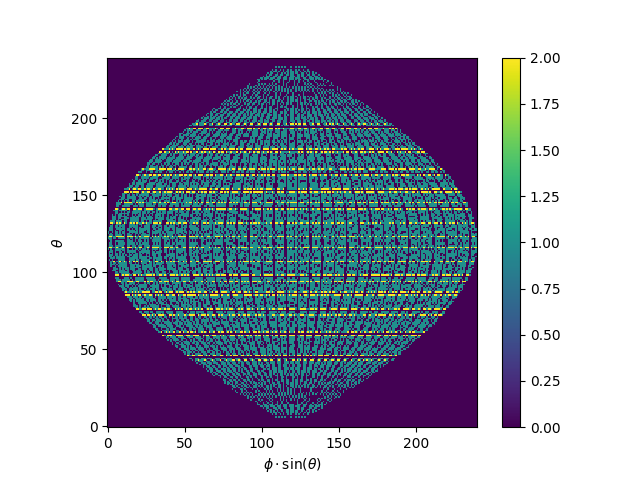
\includegraphics[width=\textwidth]{images/jcnn/pmt_repartition.png}
  \caption{Repartition of SPMTs in the image projection. The color scale is the number of SPMTs per pixel}
  \label{fig:jcnn:pmt_rep}
\end{figure}

\begin{figure}[ht]
  \begin{subfigure}[t]{0.48\linewidth}
    \centering
    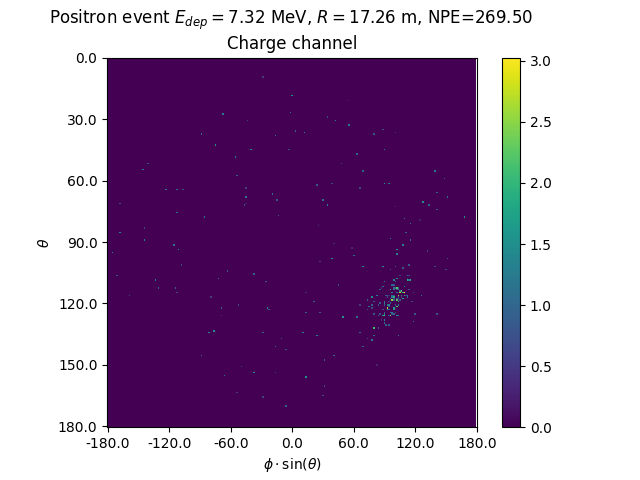
\includegraphics[width=\textwidth]{images/jcnn/illustration_0_charge.png}
  \end{subfigure}
  \hfill
  \begin{subfigure}[t]{0.48\linewidth}
    \centering
    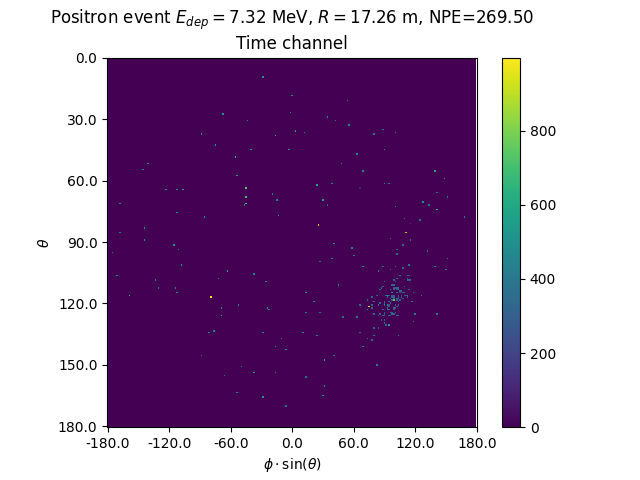
\includegraphics[width=\textwidth]{images/jcnn/illustration_0_time.png}
  \end{subfigure}
  \caption{Example of a high energy, radial event. We see a concentration of the charge on the bottom right of the image, clear indication of a high radius event. \textbf{On the left}: the charge channel. The color is the charge in each pixel in NPE equivalent. \textbf{On the right}: The time channel in nanoseconds.}
  \label{fig:jcnn:event:hrhe}
\end{figure}

\begin{figure}[ht]
  \begin{subfigure}[t]{0.48\linewidth}
    \centering
    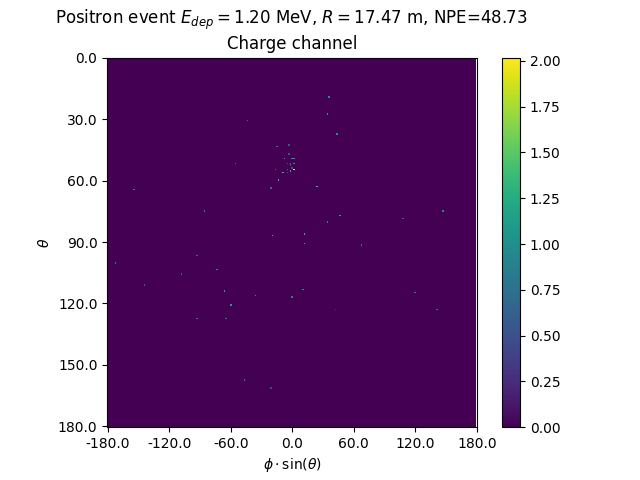
\includegraphics[width=\textwidth]{images/jcnn/illustration_1_charge.png}
  \end{subfigure}
  \hfill
  \begin{subfigure}[t]{0.48\linewidth}
    \centering
    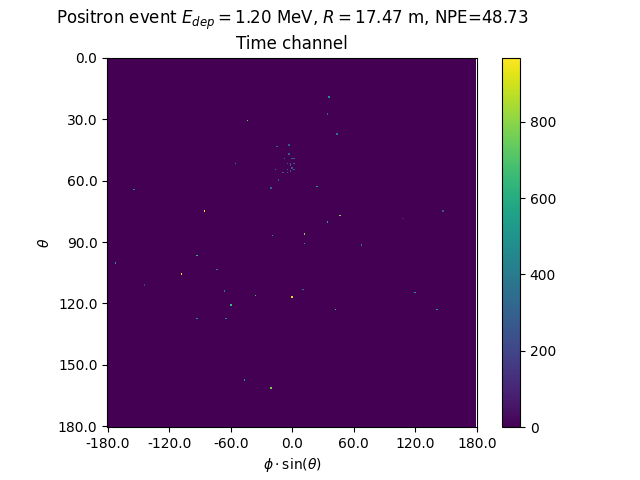
\includegraphics[width=\textwidth]{images/jcnn/illustration_1_time.png}
  \end{subfigure}
  \caption{Example of a low energy, radial event. The signal here is way less explicit, we can kind of guess that the event is located in the top middle of the image. \textbf{On the left}: the charge channel. The color is the charge in each pixel in NPE equivalent. \textbf{On the right}: The time channel in nanoseconds.}
  \label{fig:jcnn:event:hrle}
\end{figure}
\begin{figure}[ht]
  \begin{subfigure}[t]{0.48\linewidth}
    \centering
    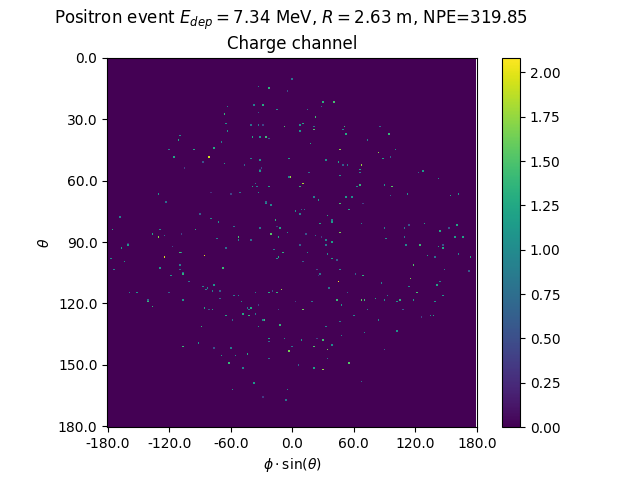
\includegraphics[width=\textwidth]{images/jcnn/illustration_2_charge.png}
  \end{subfigure}
  \hfill
  \begin{subfigure}[t]{0.48\linewidth}
    \centering
    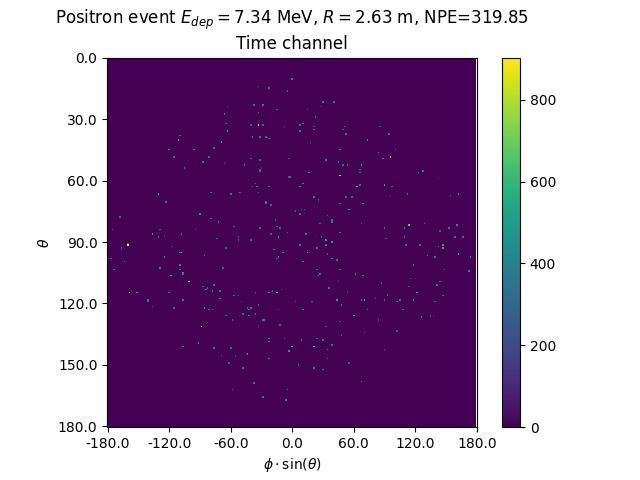
\includegraphics[width=\textwidth]{images/jcnn/illustration_2_time.png}
  \end{subfigure}
  \caption{Example of a high energy, central event. In this image we can see a lot of signal but uniformly spread, this is indicative of a central event. \textbf{On the left}: the charge channel. The color is the charge in each pixel in NPE equivalent. \textbf{On the right}: The time channel in nanoseconds.}
  \label{fig:jcnn:event:lrhe}
\end{figure}
\begin{figure}[ht]
  \begin{subfigure}[t]{0.48\linewidth}
    \centering
    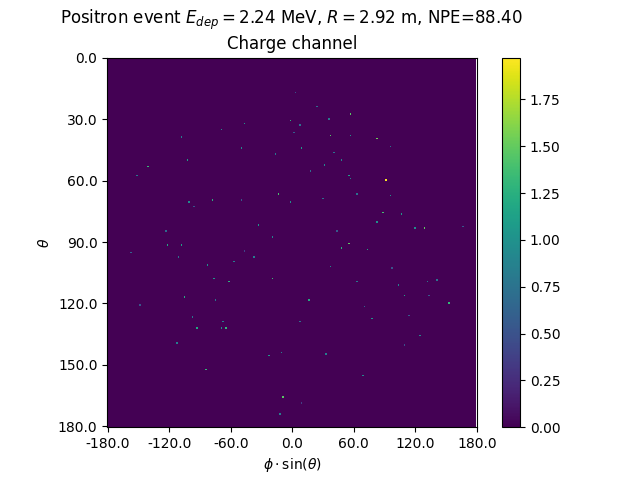
\includegraphics[width=\textwidth]{images/jcnn/illustration_3_charge.png}
  \end{subfigure}
  \hfill
  \begin{subfigure}[t]{0.48\linewidth}
    \centering
    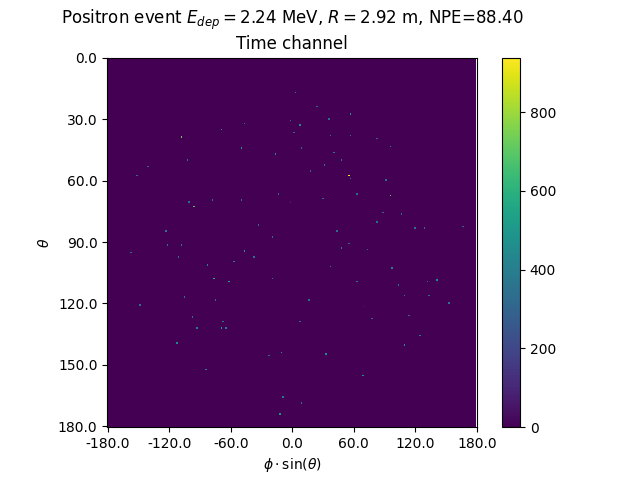
\includegraphics[width=\textwidth]{images/jcnn/illustration_3_time.png}
  \end{subfigure}
  \caption{Example of a low energy, central event. Here there is no clear signal, the uniformity of the distribution should make it central. \textbf{On the left}: the charge channel. The color is the charge in each pixel in NPE equivalent. \textbf{On the right}: The time channel in nanoseconds.}
  \label{fig:jcnn:event:lrle}
\end{figure}

In figures \ref{fig:jcnn:event:hrhe}, \ref{fig:jcnn:event:hrle}, \ref{fig:jcnn:event:lrhe} and \ref{fig:jcnn:event:lrle} are presented events from J23 for different positions and energies. We see some characteristics and we can instinctively understand how the CNN could discriminate different situations.

\begin{figure}[ht]
  \begin{subfigure}[t]{0.48\linewidth}
    \centering
    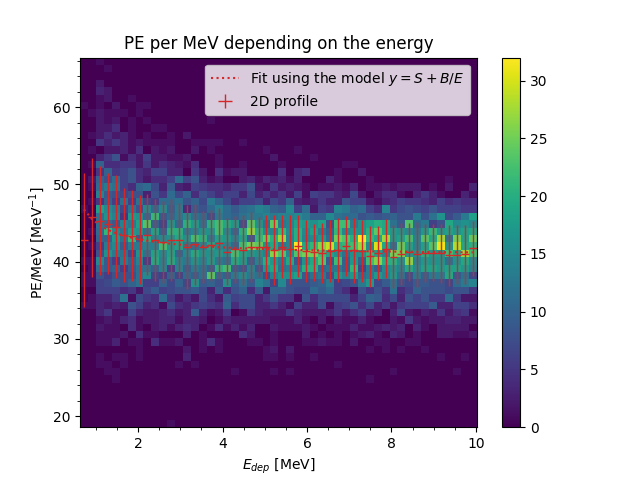
\includegraphics[width=\textwidth]{images/jcnn/pe_mev.png}
    \caption{Distribution of PE/MeV in the J23 Dataset. This distribution is profiled and fitted using equation \ref{eq:jcnn:pe_per_mev}}
    \label{fig:jcnn:pe_per_mev}
  \end{subfigure}
  \hfill
  \begin{subfigure}[t]{0.48\linewidth}
    \centering
    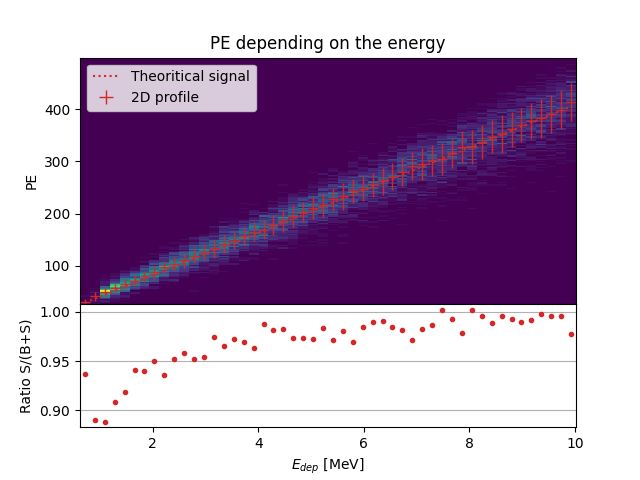
\includegraphics[width=\textwidth]{images/jcnn/pe_vs_mev.png}
    \caption{\textbf{On top}: Distribution of PE vs Energy. \textbf{On bottom}: Using the values extracted in \ref{fig:jcnn:pe_per_mev}, we calculate the ration signal over background + signal}
    \label{fig:jcnn:pe_vs_mev}
  \end{subfigure}
  \caption{}
\end{figure}

To give an idea of the strength of the signal in comparison to the dark noise background, figure \ref{fig:jcnn:pe_per_mev} present the distribution of the ration NPE over the deposited energy. Assuming a linear response of the LS we can model:
\begin{align}
  NPE_{tot} &= E_{dep} \cdot P_{mev} + D_{N} \\
  \frac{NPE_{tot}}{E_{dep}} &= P_{mev} + \frac{D_{N}}{E_{dep}} \label{eq:jcnn:pe_per_mev}
\end{align}
where $NPE_{tot}$ is the total number of PE detected by the event, $P_{mev}$ is the mean number of PE detected per MeV and $D_{N}$ is the dark noise contribution that is considered energy independent. In the case where the readout time window is dependent of the energy the dark noise contribution become energy dependant, also the LS response is realistically energy dependant but figure \ref{fig:jcnn:pe_per_mev} shows that we hare heavily dominated by statistical uncertainties which is why we are using this simple model.

The fit gives shows a light yield of 40.78 PE/MeV and a dark noise contribution of 4.29 NPE. As shown in figure \ref{fig:jcnn:pe_vs_mev}, the physics makes for 90\% of the signal at low energy.


\section{Results}

Before presenting the results, lets discuss the different observables.

The event are considered point like in this study. The target truth position, or vertex, is the mean position of the energy deposits of the positron and the two annihilation gammas. Due to the symmetries of the detector, we mainly considered and discuss the bias and precision evolution depending of the radius $R$ but we will still monitor the performances depending of the spheric angle $\theta$ and $\phi$. From the detector construction and effect we expect relative important dependencies in radius thanks to the TR area effect presented in section \ref{sec:juno:reco} and the possibility for the positron or the gammas to escape from the CD for near the edge events. We  also expect dependence in $\theta$, the top of the experiment being non-instrumented due to the filling chimney. It is also to be noted that the events in the dataset are uniformly distributed in the CD, and so are uniformly distributed in $R^3$ and $\phi$. The $\theta$ distribution is not uniform and we will have more event for $\theta \sim 90^{\circ}$ that $\theta \sim 0^{\circ}$ or $\theta \sim 180^{\circ}$.

We define multiple energy in JUNO:
\begin{itemize}
  \item $E_\nu$: The energy of the neutrino.
  \item $E_k$: The kinetic energy of the resulting positron from the IBD.
  \item $E_{dep}$: The deposited energy of the positron and the two annihilation gammas.
  \item $E_{vis}$: The equivalent visible energy, so $E_{dep}$ after the detector effect such as the absorption of scintillation photons by the LS and the LS response non-linearity.
  \item $E_{rec}$: The reconstructed energy by the reconstruction algorithm. The expected value depend on the algorithm we discuss about. For example the algorithm presented in section \ref{sec:juno:reco} is reconstructing $E_{rec}$ while the ones presented in section \ref{sec:juno:ml} reconstruct $E_{dep}$.
\end{itemize}

In this study, we will set $E_{rec}$ as our target for energy reconstruction. This choice is motivated by the ease with which we can retrieve this information in the monte-carlo data while $E_{vis}$ is less trivial to retrieve.

\subsection{J21 results}

Those results comes from the ``gen\_30'' model, meaning then 30th model generated using the table \ref{tab:jcnn:hyper} or
\begin{itemize}
 \item ``gen\_30'': $N_{blocks} = 3$, $N_{channels} = 32$, FCDNN configuration: 2048 * 2 + 1024 * 2, Loss $\coloneq E+V$
\end{itemize}

The performances of its reconstruction are presented in blue in figure \ref{fig:jcnn:vic_cnn}. Superimposed in black is the performances of the classical algorithm from \cite{lebrin_towards_2022}.

\subsubsection{Energy reconstruction}

By looking at the figure \ref{fig:jcnn:vic_cnn:multi_vic_cnn_MESBvETC} and \ref{fig:jcnn:vic_cnn:multi_vic_cnn_MESBvRTC}, the CNN has similar performances in its energy resolution. Only at the end of the energy range does the resolution get a little better.

This is explained by looking at the true and reconstructed energy distributions in figure \ref{fig:jcnn:edis}. We see that the distributions are similar for energies before 8 MeV but there is an excess of event reconstructed with energies around 9 MeV while a lack of them for 10 MeV. The neural network seems to learn the energy distribution and learn that it exist almost no event with an energy inferior to 1.022 MeV and not event with an energy superior to 10 MeV.

The first observation is a physics phenomena: for a positron, its minimum deposited energy is the mass energy coming from its annihilation with an electron 1.022 MeV. There is a few event with energies inferior to 1.022 MeV, in those case the annihilation gammas or even the positron escape the detector. The deposited energy in the LS is thus only a fraction of the energy is deposited.

The second observation is indeed true in this dataset but has no physical meaning, it is an arbitrary limit because the physics region of interest is mainly between 1 and 9 MeV of deposited energy (figure \ref{fig:juno:juno-spectrum-oscillation}). By learning the energy distribution, the CNN pull event from the border of it to more central value. That's why the energy resolution is better: the events are pulled in a small energy region , thus a small variance but the bias become very high (figure \ref{fig:jcnn:vic_cnn:multi_vic_cnn_MESBvETC}).


\begin{figure}[ht]
  \centering
  \begin{subfigure}[t]{0.32\linewidth}
    \centering
    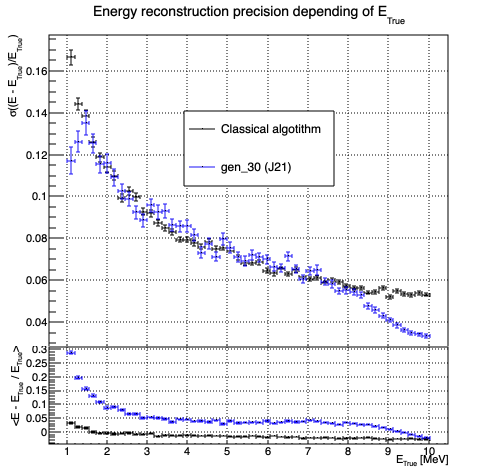
\includegraphics[width=\linewidth]{images/jcnn/vic_cnn/multi_vic_cnn_MESBvETC.png}
    \caption{Resolution and bias of energy reconstruction vs energy}
    \label{fig:jcnn:vic_cnn:multi_vic_cnn_MESBvETC}
  \end{subfigure}
  \begin{subfigure}[t]{0.32\linewidth}
    \centering
    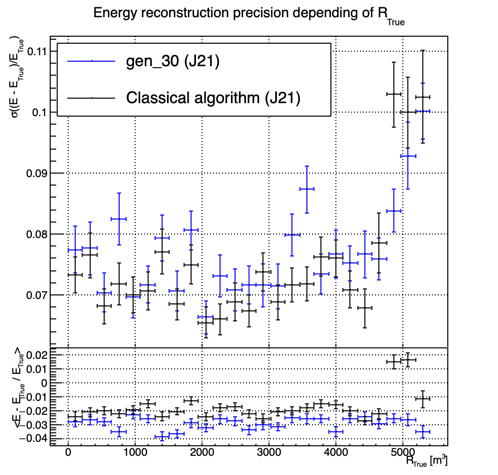
\includegraphics[width=\linewidth]{images/jcnn/vic_cnn/multi_vic_cnn_MESBvRTC.png}
    \caption{Resolution and bias of energy reconstruction vs radius}
    \label{fig:jcnn:vic_cnn:multi_vic_cnn_MESBvRTC}
  \end{subfigure}
  \begin{subfigure}[t]{0.32\linewidth}
    \centering
    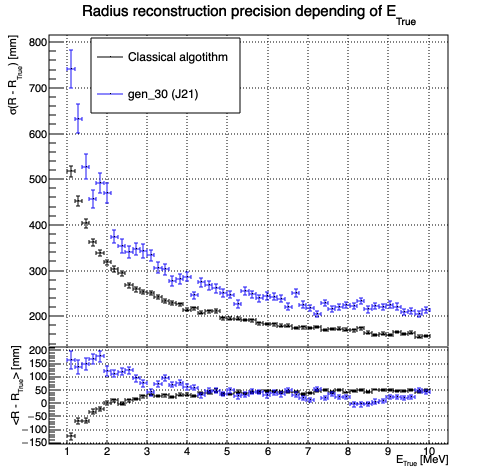
\includegraphics[width=\linewidth]{images/jcnn/vic_cnn/multi_vic_cnn_MSBvETC.png}
    \caption{Resolution and bias of radius reconstruction vs energy}
    \label{fig:jcnn:vic_cnn:multi_vic_cnn_MSBvETC}
  \end{subfigure}


  \begin{subfigure}[t]{0.32\linewidth}
    \centering
    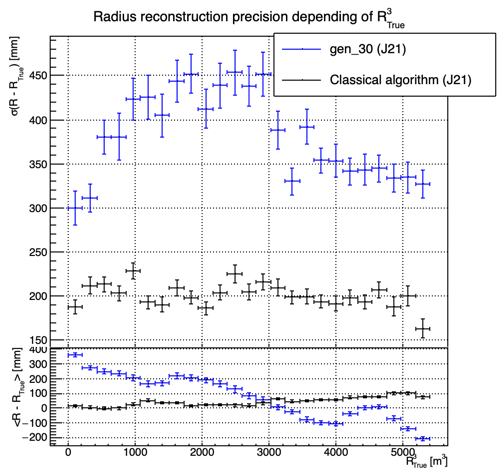
\includegraphics[width=\linewidth]{images/jcnn/vic_cnn/multi_vic_cnn_MSBvRTC.png}
    \caption{Resolution and bias of radius reconstruction vs radius}
    \label{fig:jcnn:vic_cnn:multi_vic_cnn_MSBvRTC}
  \end{subfigure}
  \begin{subfigure}[t]{0.32\linewidth}
    \centering
    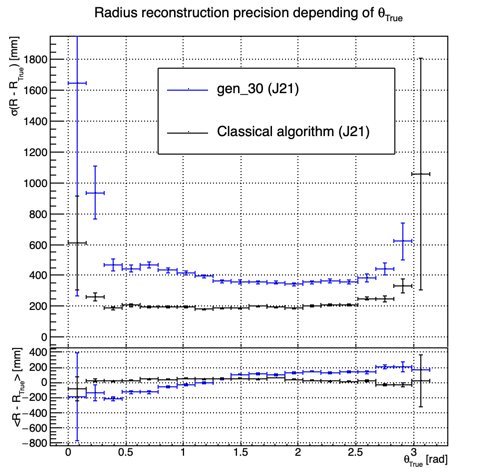
\includegraphics[width=\linewidth]{images/jcnn/vic_cnn/multi_vic_cnn_MSBvTTC.png}
    \caption{Resolution and bias of radius reconstruction vs $\theta$}
    \label{fig:jcnn:vic_cnn:multi_vic_cnn_MSBvTTC}
  \end{subfigure}
  \begin{subfigure}[t]{0.32\linewidth}
    \centering
    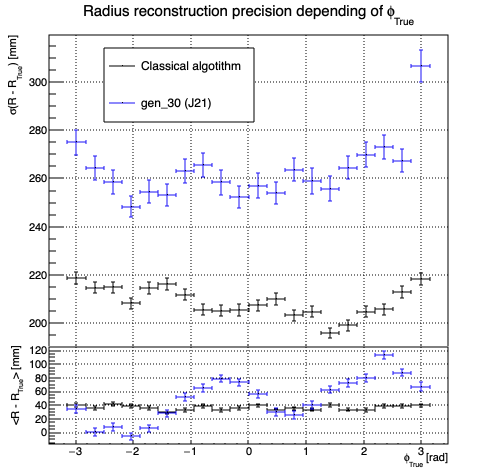
\includegraphics[width=\linewidth]{images/jcnn/vic_cnn/multi_vic_cnn_MSBvPTC.png}
    \caption{Resolution and bias of radius reconstruction vs $\phi$}
    \label{fig:jcnn:vic_cnn:multi_vic_cnn_MSBvPTC}
  \end{subfigure}
  \caption{Reconstruction performance of the ``gen\_30'' model on J21 data and it's comparison to the performances of the classic algorithm ``Classical algorithm'' from \cite{lebrin_towards_2022}. The top part of each plot is the resolution and the bottom part is the bias.}
  \label{fig:jcnn:vic_cnn}
\end{figure}

This behavior also explain the heavy bias at low energy in figure \ref{fig:jcnn:vic_cnn:multi_vic_cnn_MESBvETC}. The energy bias of the CNN if fairly constant over the energy range, it is interesting to note that the energy bias depending on the radius is a bit worse than the classical method.

\subsubsection{Vertex reconstruction}

For the vertex reconstruction we do not study $x$, $y$ and $z$ independently but we use $R$ as a proxy observable. Figure \ref{fig:jcnn:vic_cnn:cnn_perf} shows the error distribution of the different vertex coordinates. We see that $R$ errors and biases are slightly superior to the cartesian coordinates, thus $R$ is a conservative proxy observable to discuss the subject of vertex reconstruction.

The comparison of radius reconstruction between the classical algorithm and ``gen\_30'' are presented in the figures \ref{fig:jcnn:vic_cnn:multi_vic_cnn_MSBvETC}, \ref{fig:jcnn:vic_cnn:multi_vic_cnn_MSBvRTC}, \ref{fig:jcnn:vic_cnn:multi_vic_cnn_MSBvTTC} and \ref{fig:jcnn:vic_cnn:multi_vic_cnn_MSBvPTC}.

Radius reconstruction is worse than the classical algorithms in all configuration. In energy, figure \ref{fig:jcnn:vic_cnn:multi_vic_cnn_MSBvETC}, where we see a degradation of almost 20cm over the energy range.

When looking over the true event radius, figure \ref{fig:jcnn:vic_cnn:multi_vic_cnn_MSBvRTC}, we lose between 30 and 45cm of resolution. The performances the best for central and radial event.

The precision also worsen when looking at the edge of the image $\theta \approx 0$, $\theta \approx 2\pi$ respectively the top and bottom of the image, and when $\phi \approx -\pi$ and $\phi \approx \pi$ respectively the left and right side of the image. This is the confirmation that the deformation of the image is problematic for the event reconstruction.

The bias in radius reconstruction is about the same order of magnitude depending of the energy but is of opposite sign. As for the energy, this behavior is studied in more details in section \ref{sec:jcnn:combination}. Over radius, $\theta$ and $\phi$ the bias is inconsistent, sometimes event better than the classical reconstruction and but also can much worse than the classical method. This could come from the specialisation of some filters in the convolutional layers for specific part of the detector that would still work ``correctly'' for close part but with much less precision.

\begin{figure}[ht]
  \centering
  \begin{subfigure}[t]{0.32\linewidth}
    \centering
    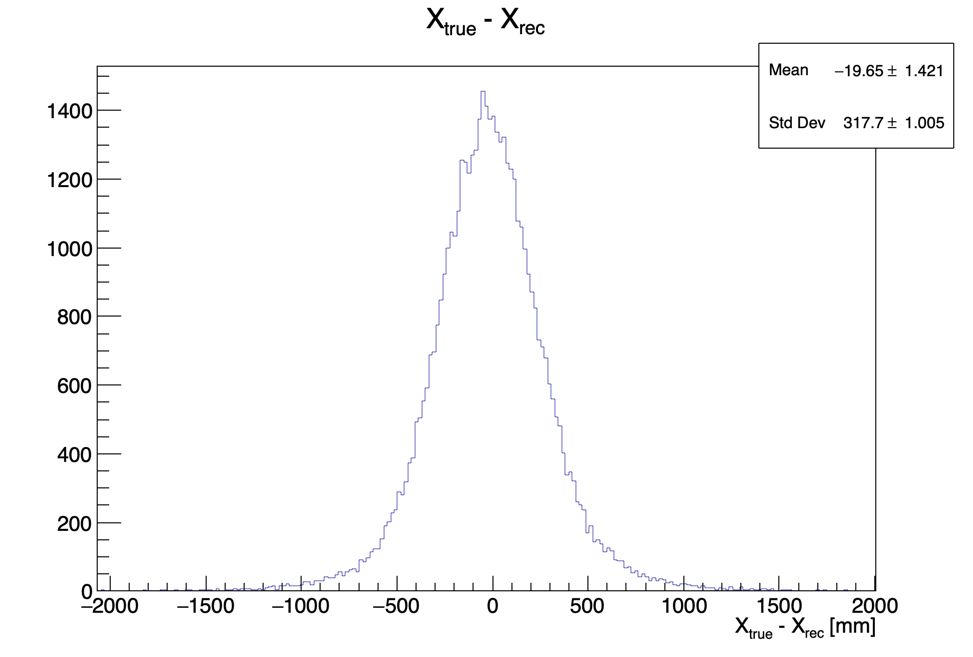
\includegraphics[width=\linewidth]{images/jcnn/vic_cnn/cnn_delta_x.png}
    \caption{Distribution of the error on reconstructed $x$ by ``gen\_30''}
    \label{fig:jcnn:vic_cnn:cnn_delta_x}
  \end{subfigure}
  \begin{subfigure}[t]{0.32\linewidth}
    \centering
    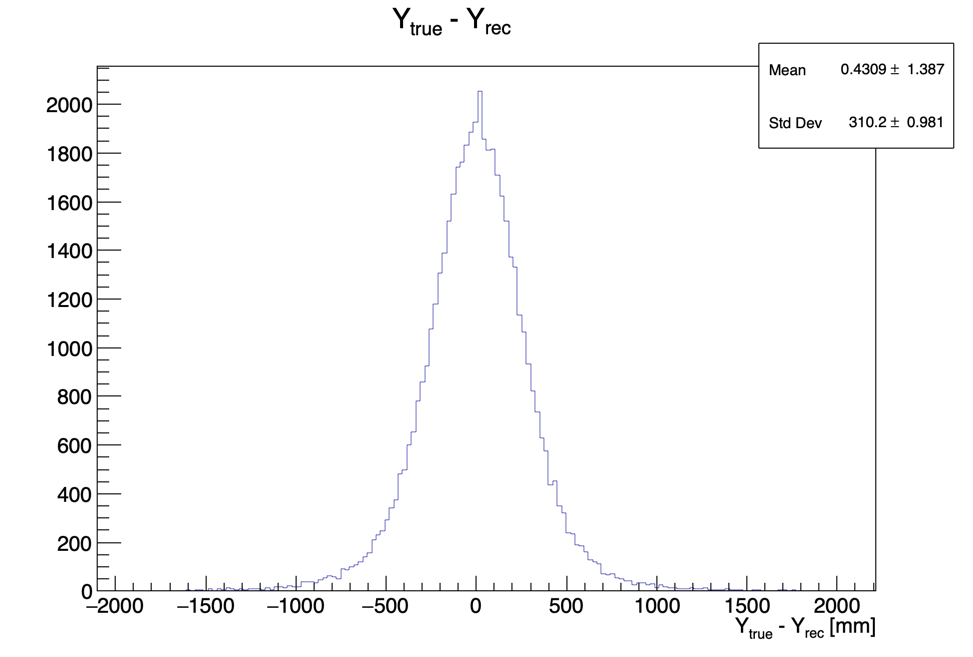
\includegraphics[width=\linewidth]{images/jcnn/vic_cnn/cnn_delta_y.png}
    \caption{Distribution of the error on reconstructed $y$ by ``gen\_30''}
    \label{fig:jcnn:vic_cnn:cnn_delta_y}
  \end{subfigure}
  \begin{subfigure}[t]{0.32\linewidth}
    \centering
    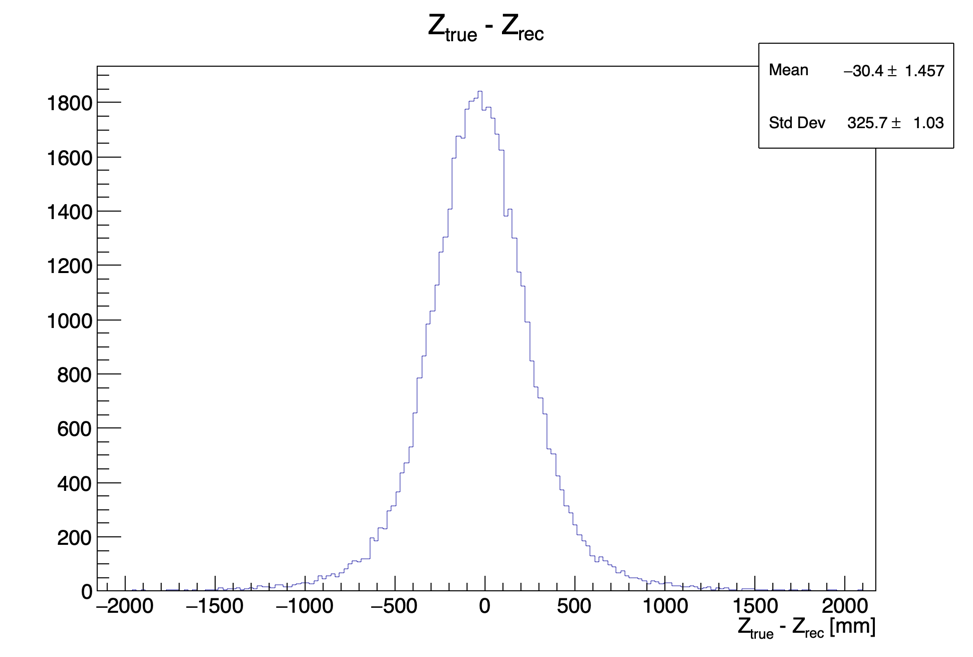
\includegraphics[width=\linewidth]{images/jcnn/vic_cnn/cnn_delta_z.png}
    \caption{Distribution of the error on reconstructed $z$ by ``gen\_30''}
    \label{fig:jcnn:vic_cnn:cnn_delta_z}
  \end{subfigure}


  \begin{subfigure}[t]{0.32\linewidth}
    \centering
    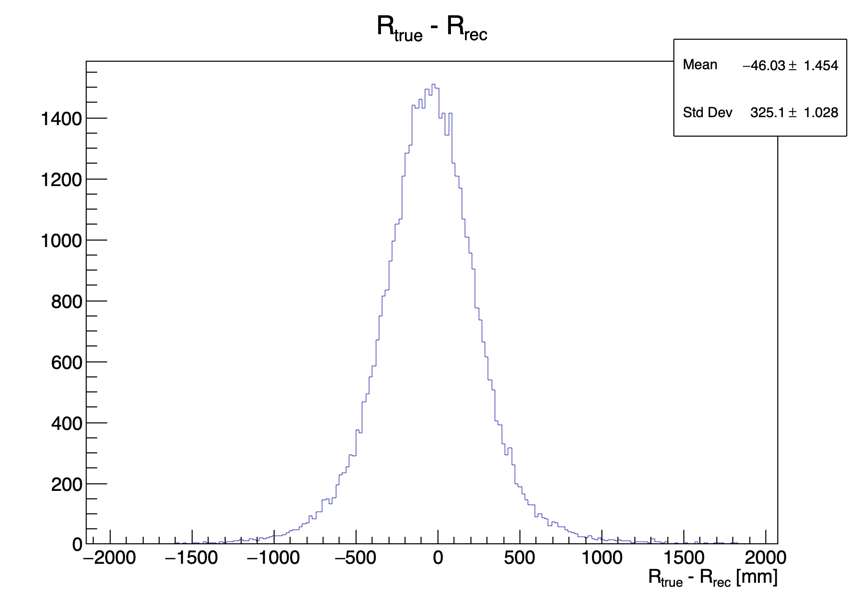
\includegraphics[width=\linewidth]{images/jcnn/vic_cnn/cnn_delta_r.png}
    \caption{Distribution of the error on reconstructed $R$ by ``gen\_30''}
    \label{fig:jcnn:vic_cnn:cnn_delta_r}
  \end{subfigure}
  \begin{subfigure}[t]{0.32\linewidth}
    \centering
    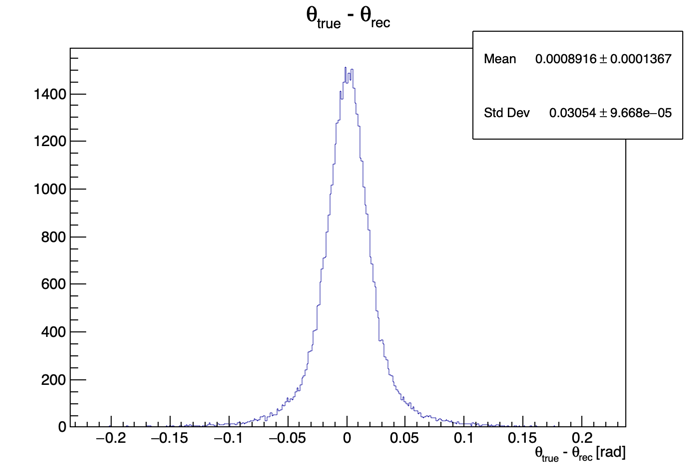
\includegraphics[width=\linewidth]{images/jcnn/vic_cnn/cnn_delta_theta.png}
    \caption{Distribution of the error on reconstructed $\theta$ by ``gen\_30''}
    \label{fig:jcnn:vic_cnn:cnn_delta_theta}
  \end{subfigure}
  \begin{subfigure}[t]{0.32\linewidth}
    \centering
    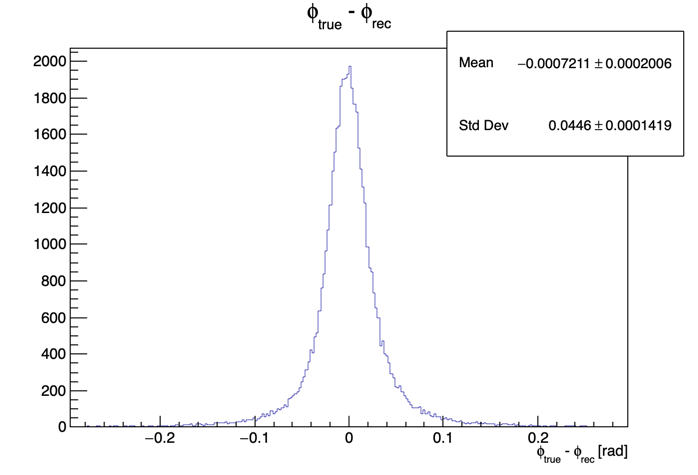
\includegraphics[width=\linewidth]{images/jcnn/vic_cnn/cnn_delta_phi.png}
    \caption{Distribution of the error on reconstructed $\phi$ by ``gen\_30''}
    \label{fig:jcnn:vic_cnn:cnn_delta_phi}
  \end{subfigure}
  \caption{Error distribution of the different component of the vertex by ``gen\_30''. The reconstructed component are $x$, $y$ and $z$ but we see similar behavior in the error of $R$, $\theta$ and $\phi$.}
  \label{fig:jcnn:vic_cnn:cnn_perf}
\end{figure}

\begin{figure}[ht]
  \centering
  \begin{subfigure}[t]{0.48\linewidth}
    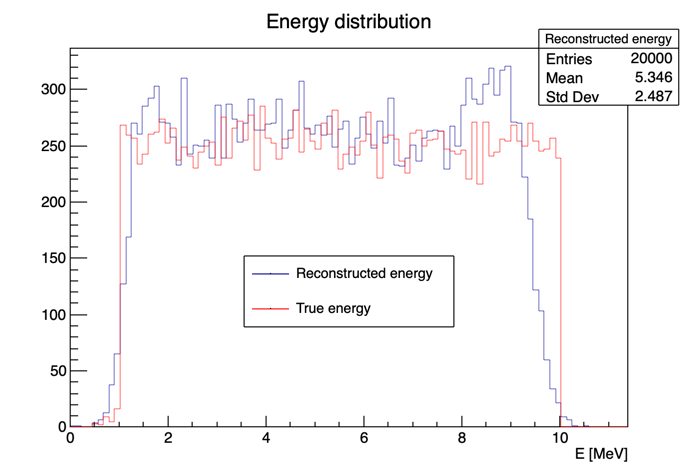
\includegraphics[width=\linewidth]{images/jcnn/vic_cnn/e_dis.png}
    \caption{Distribution of ``gen\_30'' reconstructed energy and true energy of the analysis dataset (J21)}
    \label{fig:jcnn:edis}
  \end{subfigure}
  \hfill
  \begin{subfigure}[t]{0.48\linewidth}
    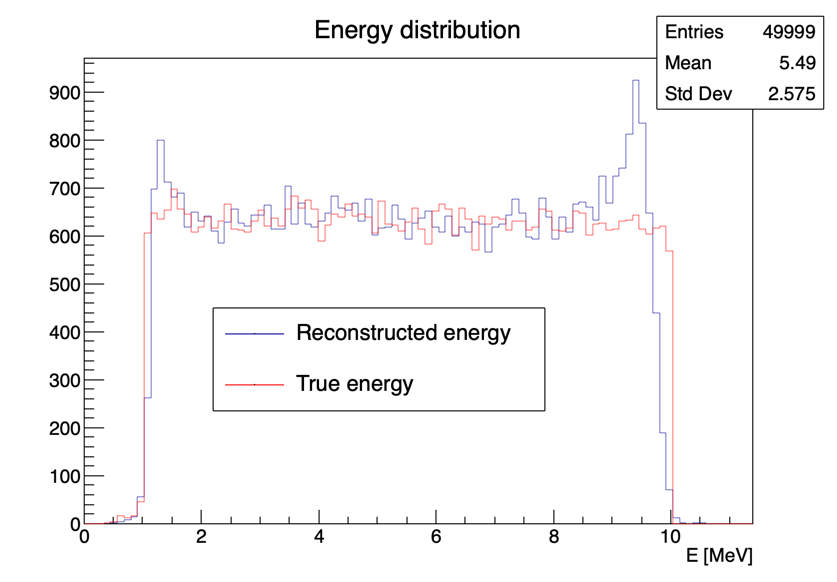
\includegraphics[width=\linewidth]{images/jcnn/vic_cnn/e_dis_42.png}
    \caption{Distribution of ``gen\_42'' reconstructed energy and true energy of the analysis dataset (J23)}
    \label{fig:jcnn:edis42}
  \end{subfigure}
  \caption{}
\end{figure}


\subsection{Combination of classic and ML estimator}
\label{sec:jcnn:combination}

%\begin{itemize}
%  \item We want to reconstruct the E from $\bar{\nu_e}$
%  \item Difference between multiple E -> $E_{vis}$, $E_{rec}$, $E_k$
%  \item Comparison with victor results
%  \item \textbf{More details when I'll look into the retrained data}
%  \item Discuss of the differences
%  \item Discuss of the principle of error decorelation
%    \begin{itemize}
%      \item Possible improvements
%      \item Combining algorithms
%      \item Average sum
%    \end{itemize}
%\end{itemize}

As it has been presented in previous section, there is instances where the reconstructed energy and vertex behaves differently between the neural network and  the classic algorithm. For instance, if we look at figure \ref{fig:jcnn:vic_cnn:multi_vic_cnn_MSBvETC}, we see that while the CNN tend to overestimate the at low energy, the classical algorithm seems to underestimate this radius. Let's designate the two reconstruction algorithms as estimator of $X$, the truth about the event in the phase space $(E, x, y, z)$. The CNN and the classical algorithm are respectively designated as $\theta_{N}(X)$ and $\theta_{C}(X)$.
\begin{align}
  E[\theta_{N}] = \mu_N + X; ~&~ \mathrm{Var}[\theta_{N}] = \sigma^2_{N} \\
  E[\theta_{C}] = \mu_C + X; ~&~ \mathrm{Var}[\theta_{C}] = \sigma^2_{C}
\end{align}
where $\mu$ is the bias of the estimator and $\sigma^2$ its variance.

Now if we were to combine the two esitmators using a simple mean
\begin{equation}
  \label{eq:jcnn:combi}
  \hat{\theta}(X) = \frac{1}{2} ( \theta_{N}(X) + \theta_{C}(X) ) \\
\end{equation}
then the variance and mean would follow
\begin{align}
  E[\hat{\theta}] & = \frac{1}{2}E[\theta_N] + \frac{1}{2}E[\theta_X]\\
                  & = \frac{1}{2}(\mu_N + X + \mu_C + X) \\
                  & = \frac{1}{2}(\mu_N + \mu_C) + X
\end{align}
\begin{align}
  \mathrm{Var}[\hat{\theta}] & = \frac{1}{4}\sigma^2_N + \frac{1}{4}\sigma^2_C + 2 \cdot \frac{1}{4} \cdot \sigma_{NC} \\
                             & = \frac{1}{4}\sigma^2_N + \frac{1}{4}\sigma^2_C + \frac{1}{2} \cdot \sigma_{NC} \\
                             & = \frac{1}{4}\sigma^2_N + \frac{1}{4}\sigma^2_C + \frac{1}{2} \cdot \sigma_{N} \sigma_C \rho_{NC}
\end{align}
Where $\sigma_{NC}$ is the covariance between $\theta_N$ and $\theta_C$ and $\rho_{NC}$ their correlation.

We see immediately that if the two estimators are of opposite bias, the bias of the resulting estimator is reduced. For the variance, it depends of $\rho_{NC}$ but in this case if $\sigma^2_C$ is close to $\sigma^2_N$ then even for $\rho_{NC} \lneq 1$ then we can gain in resolution.

By generalising the equation \ref{eq:jcnn:combi} to
\begin{equation}
  \hat{\theta}(X) = \alpha \theta_N + (1 - \alpha) \theta_C; ~ \alpha \in [0, 1]
\end{equation}
we can determine an optimal $\alpha$ for two combined estimators. The estimators with the smallest variance
\begin{equation}
  \alpha = \frac{\sigma_C^2 - \sigma_N \sigma_C \rho_CN}{\sigma_N^2 + \sigma_C^2 - 2\sigma_N \sigma_C \rho_NC}
\end{equation}
and the estimator without bias
\begin{equation}
  \alpha = \frac{\mu_C}{\mu_C - \mu_N}
\end{equation}
See annex \ref{sec:annex:jcnn:alpha} for demonstration.

Its pretty clear from the results shown in figure \ref{fig:jcnn:vic_cnn} that the bias, variances and correlation are not constant across the $(E, R^3)$ phase space. We thus compute those parameters in a grid in $E$ and $R^3$ for the following results as illustrated in \ref{fig:jcnn:vic_cnn:res_map}.

The map we are using are composed of 20 bins for $R^3$ going from 0 to 5400 m$^3$ (17.54 m) and 50 bins in energy ranging from 1.022 to 10.022 MeV. In the case where we are outside the grid, we use the closest cell.

\begin{figure}
  \centering
  \begin{subfigure}[t]{0.48\linewidth}
    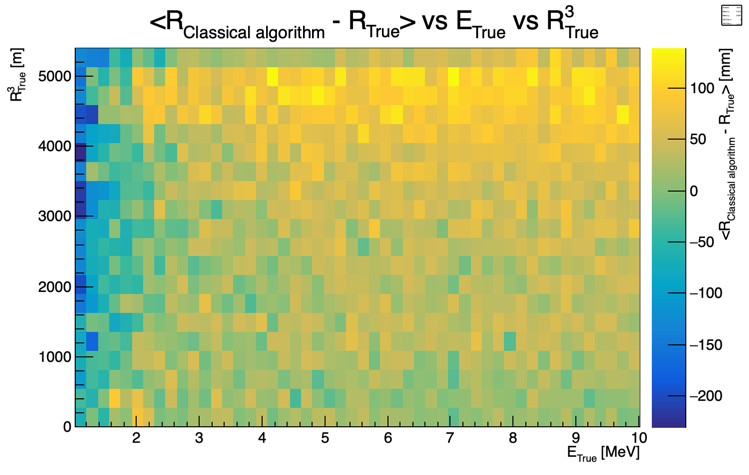
\includegraphics[width=\linewidth]{images/jcnn/vic_cnn/vic_r_bias.png}
  \end{subfigure}
  \hfill
  \begin{subfigure}[t]{0.48\linewidth}
    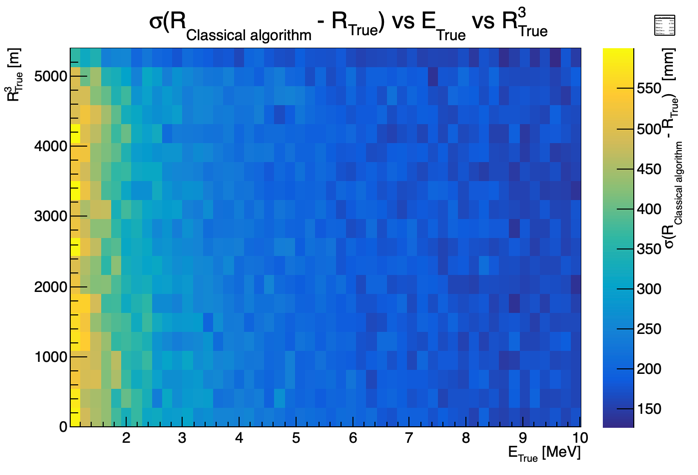
\includegraphics[width=\linewidth]{images/jcnn/vic_cnn/vic_r_res.png}
  \end{subfigure}
  \caption{Radius bias (\textbf{on the left}) and resolution(\textbf{on the right}) of the classical algorithm in a $E$, $R^3$ grid}
  \label{fig:jcnn:vic_cnn:res_map}
\end{figure}


The performance of this weighted mean is presented in figure \ref{fig:jcnn:vic_cnn:Cx30}. We can see that even when the CNN resolution is much worse than the classical algorithm, it can still bring some information thus improving the resolution. This comes from the correlation of the reconstruction error to be smaller than 1 as presented in figure \ref{fig:jcnn:vic_cnn:corr}. We even see some anticorrelation in the radius reconstruction for High radius, high energy, event.


\begin{figure}[ht]
  \centering
  \begin{subfigure}[t]{0.32\linewidth}
    \centering
    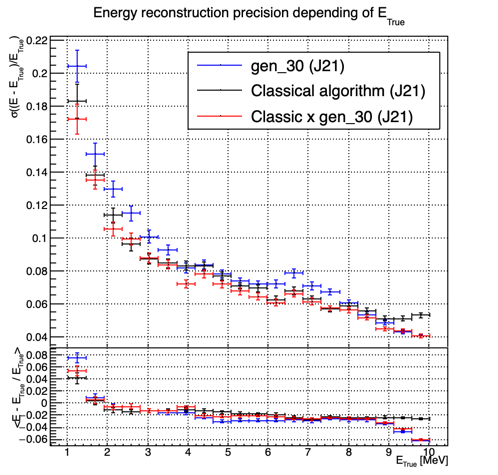
\includegraphics[width=\linewidth]{images/jcnn/vic_cnn/multi_vic_cnn_Cx30_MESBvETC.png}
    \caption{Resolution and bias of energy reconstruction vs energy}
    \label{fig:jcnn:vic_cnn:multi_vic_cnn_Cx30_MESBvETC}
  \end{subfigure}
  \begin{subfigure}[t]{0.32\linewidth}
    \centering
    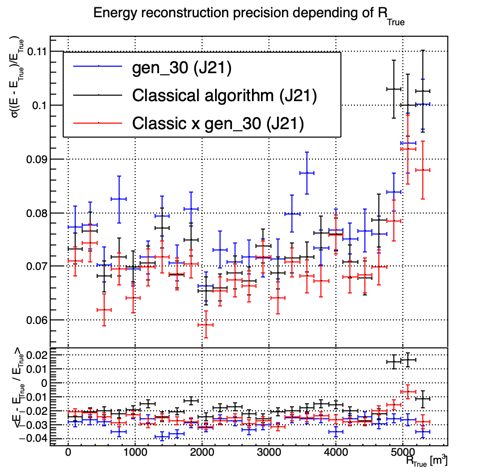
\includegraphics[width=\linewidth]{images/jcnn/vic_cnn/multi_vic_cnn_Cx30_MESBvRTC.png}
    \caption{Resolution and bias of energy reconstruction vs radius}
    \label{fig:jcnn:vic_cnn:multi_vic_cnn_Cx30_MESBvRTC}
  \end{subfigure}
  \begin{subfigure}[t]{0.32\linewidth}
    \centering
    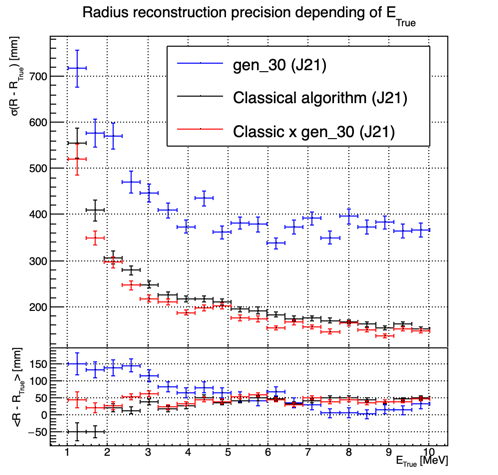
\includegraphics[width=\linewidth]{images/jcnn/vic_cnn/multi_vic_cnn_Cx30_MSBvETC.png}
    \caption{Resolution and bias of radius reconstruction vs energy}
    \label{fig:jcnn:vic_cnn:multi_vic_cnn_Cx30_MSBvETC}
  \end{subfigure}


  \begin{subfigure}[t]{0.32\linewidth}
    \centering
    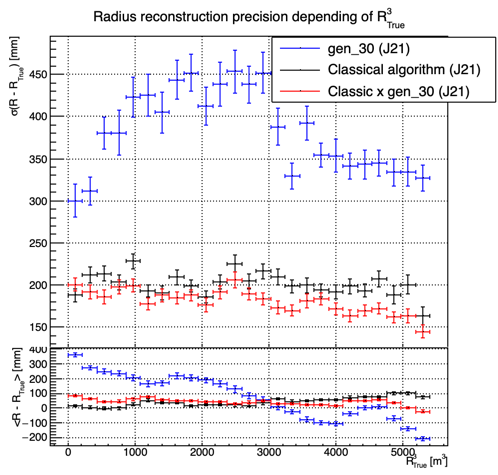
\includegraphics[width=\linewidth]{images/jcnn/vic_cnn/multi_vic_cnn_Cx30_MSBvRTC.png}
    \caption{Resolution and bias of radius reconstruction vs radius}
    \label{fig:jcnn:vic_cnn:multi_vic_cnn_Cx30_MSBvRTC}
  \end{subfigure}
  \begin{subfigure}[t]{0.32\linewidth}
    \centering
    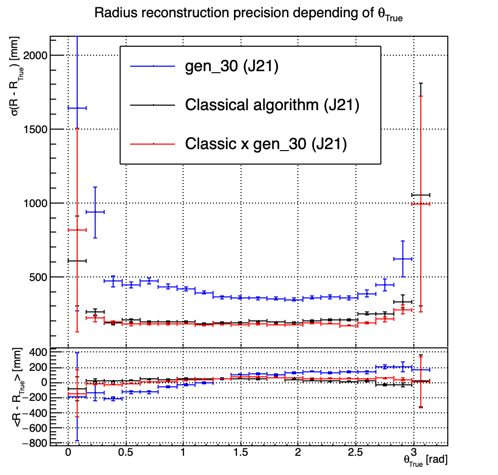
\includegraphics[width=\linewidth]{images/jcnn/vic_cnn/multi_vic_cnn_Cx30_MSBvTTC.png}
    \caption{Resolution and bias of radius reconstruction vs $\theta$}
    \label{fig:jcnn:vic_cnn:multi_vic_cnn_Cx30_MSBvTTC}
  \end{subfigure}
  \begin{subfigure}[t]{0.32\linewidth}
    \centering
    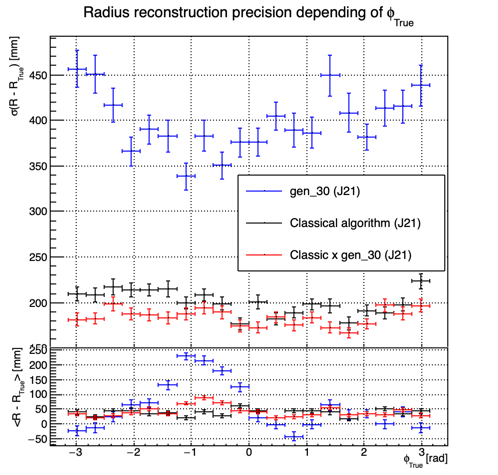
\includegraphics[width=\linewidth]{images/jcnn/vic_cnn/multi_vic_cnn_Cx30_MSBvPTC.png}
    \caption{Resolution and bias of radius reconstruction vs $\phi$}
    \label{fig:jcnn:vic_cnn:multi_vic_cnn_Cx30_MSBvPTC}
  \end{subfigure}
  \caption{Reconstruction performance of the ``gen\_30'' model on J21, the classic algorithm ``Classical algorithm'' from \cite{lebrin_towards_2022} and the combination of both using weighted mean. The top part of each plot is the resolution and the bottom part is the bias.}

  \label{fig:jcnn:vic_cnn:Cx30}
\end{figure}

\begin{figure}
  \centering
  \begin{subfigure}[t]{0.48\linewidth}
    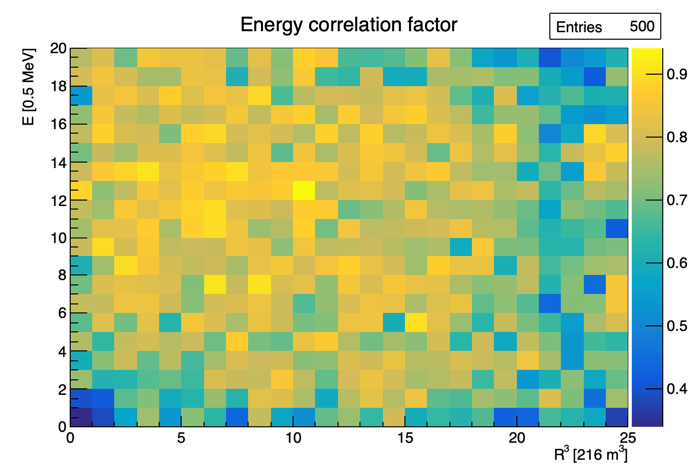
\includegraphics[width=\linewidth]{images/jcnn/vic_cnn/vic_cnn_e_corr.png}
  \end{subfigure}
  \hfill
  \begin{subfigure}[t]{0.48\linewidth}
    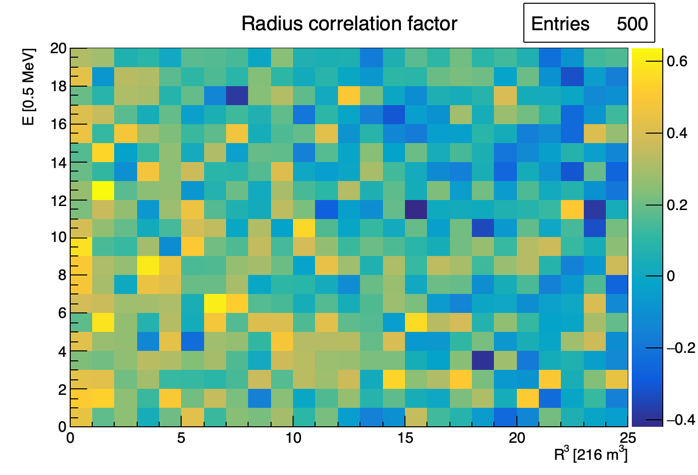
\includegraphics[width=\linewidth]{images/jcnn/vic_cnn/vic_cnn_r_corr.png}
  \end{subfigure}
  \caption{Correlation between CNN and classical method reconstruction (\textbf{on the left}) for energy and (\textbf{on the right}) for radius in a $E$, $R^3$ grid}
  \label{fig:jcnn:vic_cnn:corr}
\end{figure}

This technique is not suited for realistic reconstruction, we rely too much on the knowledge of the resolution, bias and correlation between the two methods. While this is possible to determine using simulated data or calibration sources, the real data might differ from our model and we would need to really well understand the behavior of the two system. But this is an excellent tool to indicate potential improvements to algorithms and reconstruction methods, showing with this results a potential upper limit to the reconstruction performances.

\subsection{J23 results}

The J21 simulation is fairly old and newer version, such as J23, include refined measurements of the light yield, reflection indices of materials of the detector, structural elements such as the connecting structure and more realistic dark noise. Additionally, the trigger, waveform integration and time window are defined using the algorithms that will ultimately be used by the collaboration to process real physics events.

We retrained the models defined in \ref{sec:jcnn:model} on the J23 data and used the same selection procedure. The results from the best architecture, ``gen\_42'', are presented in figure \ref{fig:jcnn:vic_cnn:gen42}. Following the table \ref{tab:jcnn:hyper}, ``gen\_42'' is defined as:
\begin{itemize}
 \item ``gen\_42'': $N_{blocks} = 3$, $N_{channels} = 64$, FCDNN configuration: 4096 * 2, Loss $\coloneq E+V$
\end{itemize}

\subsubsection{Energy reconstruction}

The results of the energy reconstruction are presented in figures \ref{fig:jcnn:vic_cnn:multi_vic_42_MESBvETC} and \ref{fig:jcnn:vic_cnn:multi_vic_42_MESBvRTC}. Similarly to what we seen for J21, the resolution is close to the one of the classical algorithm with the exception of the start and end of the spectrum. This come from ``gen\_42'' learning the shape of the distribution and pulling events from the extreme energies, like 1 and 10 MeV, to more common seen energy, like 2 and 9 MeV as illustrated in figure \ref{fig:jcnn:edis42}. The bias disappear with the exception of low and high energy events.

\subsubsection{Vertex reconstruction}

The vertex reconstruction, presented in figures \ref{fig:jcnn:vic_cnn:multi_vic_42_MSBvETC}, \ref{fig:jcnn:vic_cnn:multi_vic_42_MSBvRTC}, \ref{fig:jcnn:vic_cnn:multi_vic_42_MSBvTTC} and \ref{fig:jcnn:vic_cnn:multi_vic_42_MSBvPTC} is not yet to the level of the classical reconstruction but the degradation is smaller than for ``gen\_32'' being at most a difference of 15cm of resolution and closing to the performance of the classical algorithm in the most favourable condition. ``gen\_42'' has also very little bias in comparison with the classical method with the exception of the transition to the TR area and at the very edge of the detector.

Unfortunately could not rerun the classical algorithms over the J23 data, as the algorithm was optimised for J21 and was not included and maintained over J23. The combination method need for the two estimators to be run on the same set of event, which was impossible without the classical algorithm being maintained for J23.

Overall the resolution improved over the transition from J21 to J23, effect probably coming from a more complete and rigorous simulation.
\begin{figure}[ht]
  \centering
  \begin{subfigure}[t]{0.32\linewidth}
    \centering
    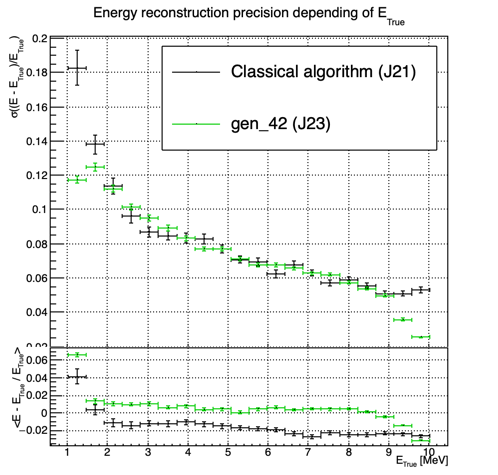
\includegraphics[width=\linewidth]{images/jcnn/vic_cnn/multi_vic_42_MESBvETC.png}
    \caption{Resolution and bias of energy reconstruction vs energy}
    \label{fig:jcnn:vic_cnn:multi_vic_42_MESBvETC}
  \end{subfigure}
  \begin{subfigure}[t]{0.32\linewidth}
    \centering
    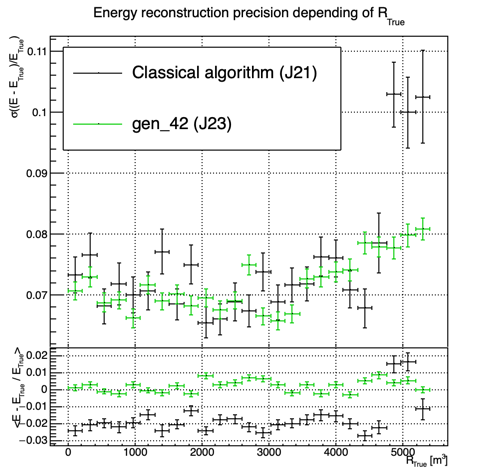
\includegraphics[width=\linewidth]{images/jcnn/vic_cnn/multi_vic_42_MESBvRTC.png}
    \caption{Resolution and bias of energy reconstruction vs radius}
    \label{fig:jcnn:vic_cnn:multi_vic_42_MESBvRTC}
  \end{subfigure}
  \begin{subfigure}[t]{0.32\linewidth}
    \centering
    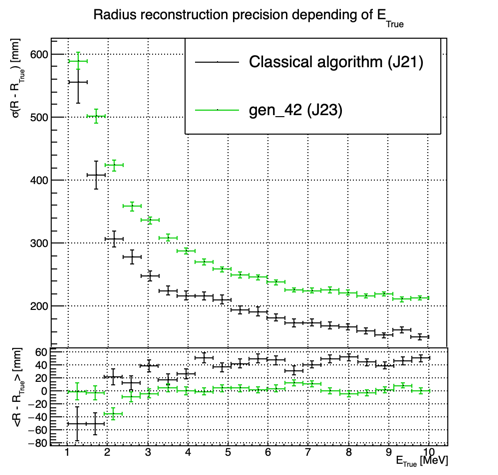
\includegraphics[width=\linewidth]{images/jcnn/vic_cnn/multi_vic_42_MSBvETC.png}
    \caption{Resolution and bias of radius reconstruction vs energy}
    \label{fig:jcnn:vic_cnn:multi_vic_42_MSBvETC}
  \end{subfigure}


  \begin{subfigure}[t]{0.32\linewidth}
    \centering
    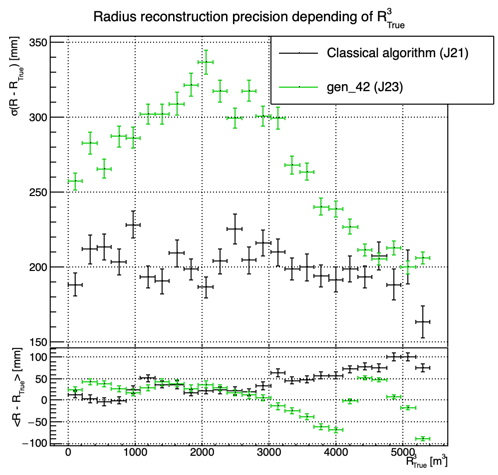
\includegraphics[width=\linewidth]{images/jcnn/vic_cnn/multi_vic_42_MSBvRTC.png}
    \caption{Resolution and bias of radius reconstruction vs radius}
    \label{fig:jcnn:vic_cnn:multi_vic_42_MSBvRTC}
  \end{subfigure}
  \begin{subfigure}[t]{0.32\linewidth}
    \centering
    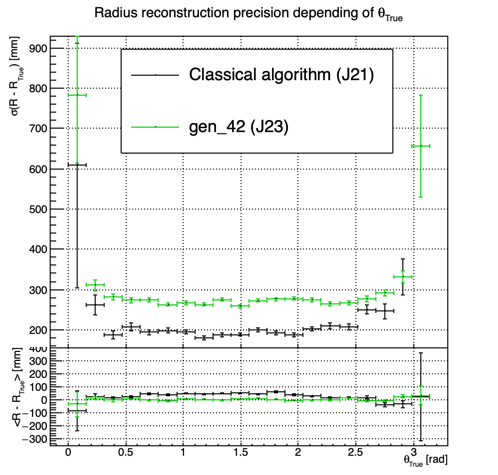
\includegraphics[width=\linewidth]{images/jcnn/vic_cnn/multi_vic_42_MSBvTTC.png}
    \caption{Resolution and bias of radius reconstruction vs $\theta$}
    \label{fig:jcnn:vic_cnn:multi_vic_42_MSBvTTC}
  \end{subfigure}
  \begin{subfigure}[t]{0.32\linewidth}
    \centering
    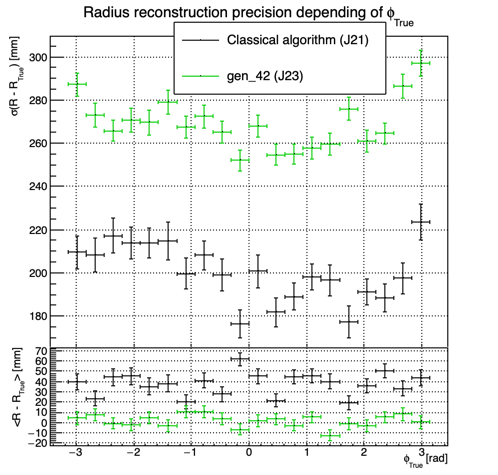
\includegraphics[width=\linewidth]{images/jcnn/vic_cnn/multi_vic_42_MSBvPTC.png}
    \caption{Resolution and bias of radius reconstruction vs $\phi$}
    \label{fig:jcnn:vic_cnn:multi_vic_42_MSBvPTC}
  \end{subfigure}
  \caption{Reconstruction performance of the ``gen\_42'' model on J23 data and it's comparison to the performances of the classic algorithm ``Classical algorithm'' from \cite{lebrin_towards_2022}. The top part of each plot is the resolution and the bottom part is the bias.}
  \label{fig:jcnn:vic_cnn:gen42}
\end{figure}

\section{Conclusion and prospect}
\label{sec:jcnn:prospect}

The CNN is a fine tool for event reconstruction in JUNO, and while the reconstruction performances are satisfactory, it show its limitation, the main one concerning the data representation. A lot of training time and resources is consumed going and optimizing over pixel with no physical meaning, the NN needs to optimized itself to take into account edges cases such as event at the edge of the image and deformation of the charge distribution.

Those problems could be circumvented, we could imagine a two part CNN where the first part reconstruct the $\theta$ and $\phi$ spherical coordinates and then rotate the image to locate the event in the center of the image. The second part, from this rotated image, would reconstruct the radius and energy of the event.

To overcome the problematic of the aggregation of PMT time information and the meaning of the time channel in case of no hit, we could transform this channel into a dimension. This would results in an image with multiple charge channels, each one representing the charge sum in a time interval.

In this thesis, we decided to solve those problem by moving away from the 2D image representation, looking into the graph representation and the Graph Neural Network (GNN). This is be the subject of the next chapter.
